\documentclass[12pt]{article}
\usepackage{graphicx}
\graphicspath{./figures/}
\usepackage[margin=1.0in]{geometry}
\usepackage{xcolor}
\definecolor{bg}{HTML}{16171e}
%\usepackage[font={color=white,bf}]{caption}
\usepackage{float}
\usepackage{amsmath}
\usepackage{url}
\usepackage{subcaption}
\usepackage{listings}

\title{MCEN 7221/ASEN 5027 Turbulence Project 2}
\author{Duncan McGough}
\date{\today}

\begin{document}
\maketitle

\tableofcontents
\listoffigures
\newpage

\section{Problem 1}
In this project report, Direct Numerical Simulation (DNS) data was taken and analyzed. Two different kinds of simulations were analyzed, one being Homogeneous Isotropic Turbulence (HIT) and the other being Homogeneous Shear Turbulence (HST). 

\subsection{Max and Min Values}
The DNS data for HIT and HST cases was put into a min/max function to find the minimum and maximum values for each velocity component in the HIT and HST fields. Noting that the data is nondimensionalized, the results are:
\begin{lstlisting}
Max HIT u: 0.8576899766921997
Max HIT v: 0.5416799783706665
Max HIT w: 0.7064499855041504
Max HST u: 5.862400054931641
Max HST v: 3.033799886703491
Max HST w: 3.131500005722046

Min HIT u: -0.7590799927711487
Min HIT v: -0.6005899906158447
Min HIT w: -0.7692000269889832
Min HST u: -5.138700008392334
Min HST v: -3.3306000232696533
Min HST w: -2.963900089263916
\end{lstlisting}

One can notice that the extreme values are in the HST case are of greater magnitude than those of the HIT case. In the HIT case, the values are generally smaller and closer together in magnitude, whereas in the HST case it is evident that the u-component has a standout larger velocity whereas the v- and w-components are similar in magnitude. This makes sense due to the nature of the simulation, as the shear has a certain imposed velocity (at least initially) that drives the flow. 

\subsection{3D Isosurfaces}
Three-dimensional isosurfaces can be created and plotted for the HIT and HST cases. When visualized, they appear as in Figure \ref{fig:iso}.

\begin{figure}
\centering
\begin{subfigure}{0.5\linewidth}
\centering
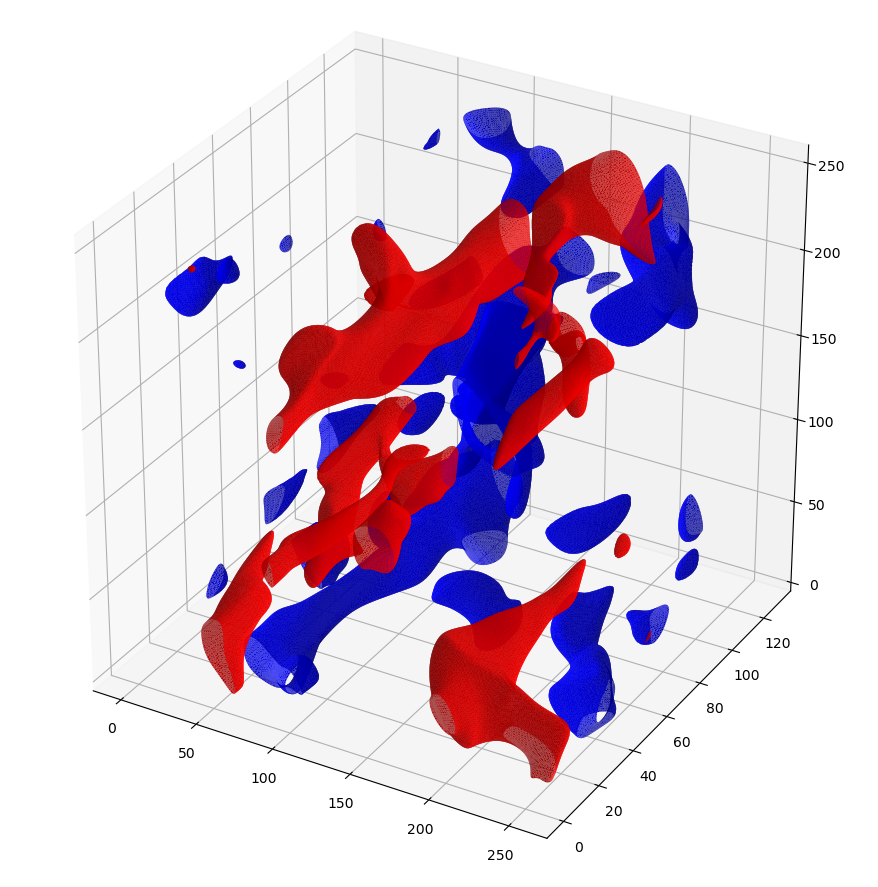
\includegraphics[width=\linewidth]{./figures/12-hit.png}
\caption{HIT}
\end{subfigure}%
\begin{subfigure}{0.5\linewidth}
\centering
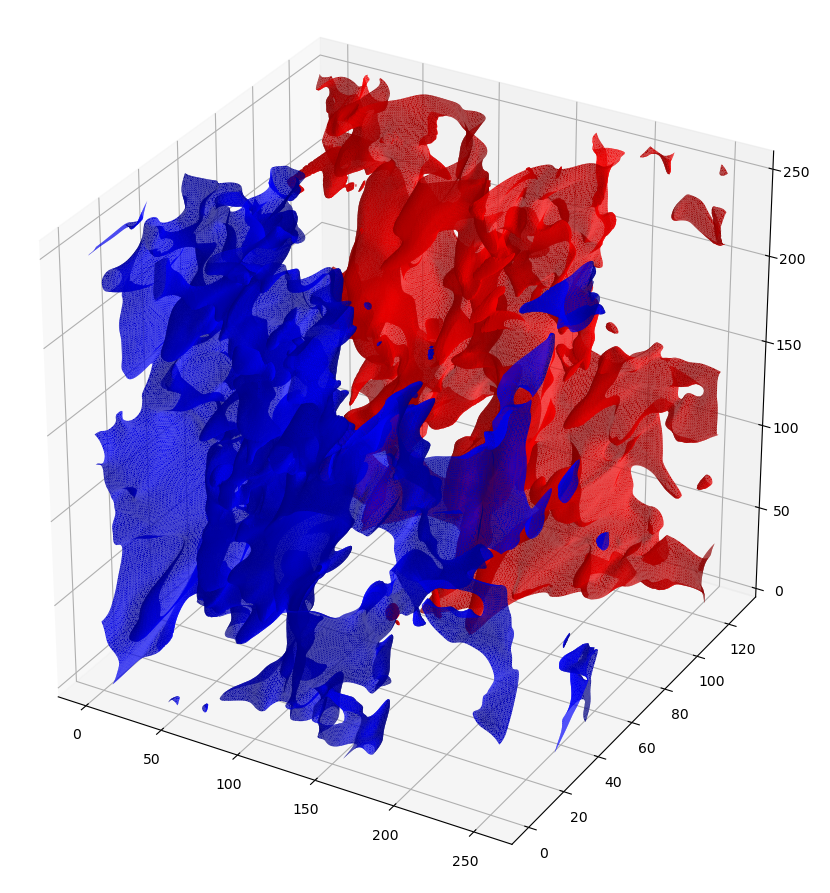
\includegraphics[width=\linewidth]{./figures/12-hst.png}
\caption{HST}
\end{subfigure}
\caption{3D Isosurfaces}
\label{fig:iso}
\end{figure}

The two colors in Figure \ref{fig:iso} represent the maximum and minimum velocities divided by two, respective to the colors blue and red. It is immediately noticeable that the HST case has a distinct division between the maximum and minimum isosurfaces, whereas the HIT case is more uniform. Another distinct feature between the cases is that HIT case has more frequent separate blob entities in a homogeneous formation of isosurfaces whereas the HST case are distinct in their shear layers. 
\subsection{Image Plane Slices}
The data can be sliced at certain planes, leaving 2D slices that can be plotted. In Figures \ref{fig:13-hit} and \ref{fig:13-hst}, the u, v, and w velocity component fields are sliced at k=[1, 128, 256] z-locations. Note that colorbar here is scaled to HST for easy comparison. Increasing slice locations are located in the columns of images whereas different velocity components are the rows of images. It is noted that u-component is the most active and polar with the velocity field in the HST data, as expected. The HIT data is more uniform and homogeneous. An interesting feature of the data is that the k=1 and k=256 planes appear identical. This is due to a repeating boundary condition that is applied to the domain of the simulation. 

\begin{figure}[H]
	\centering
	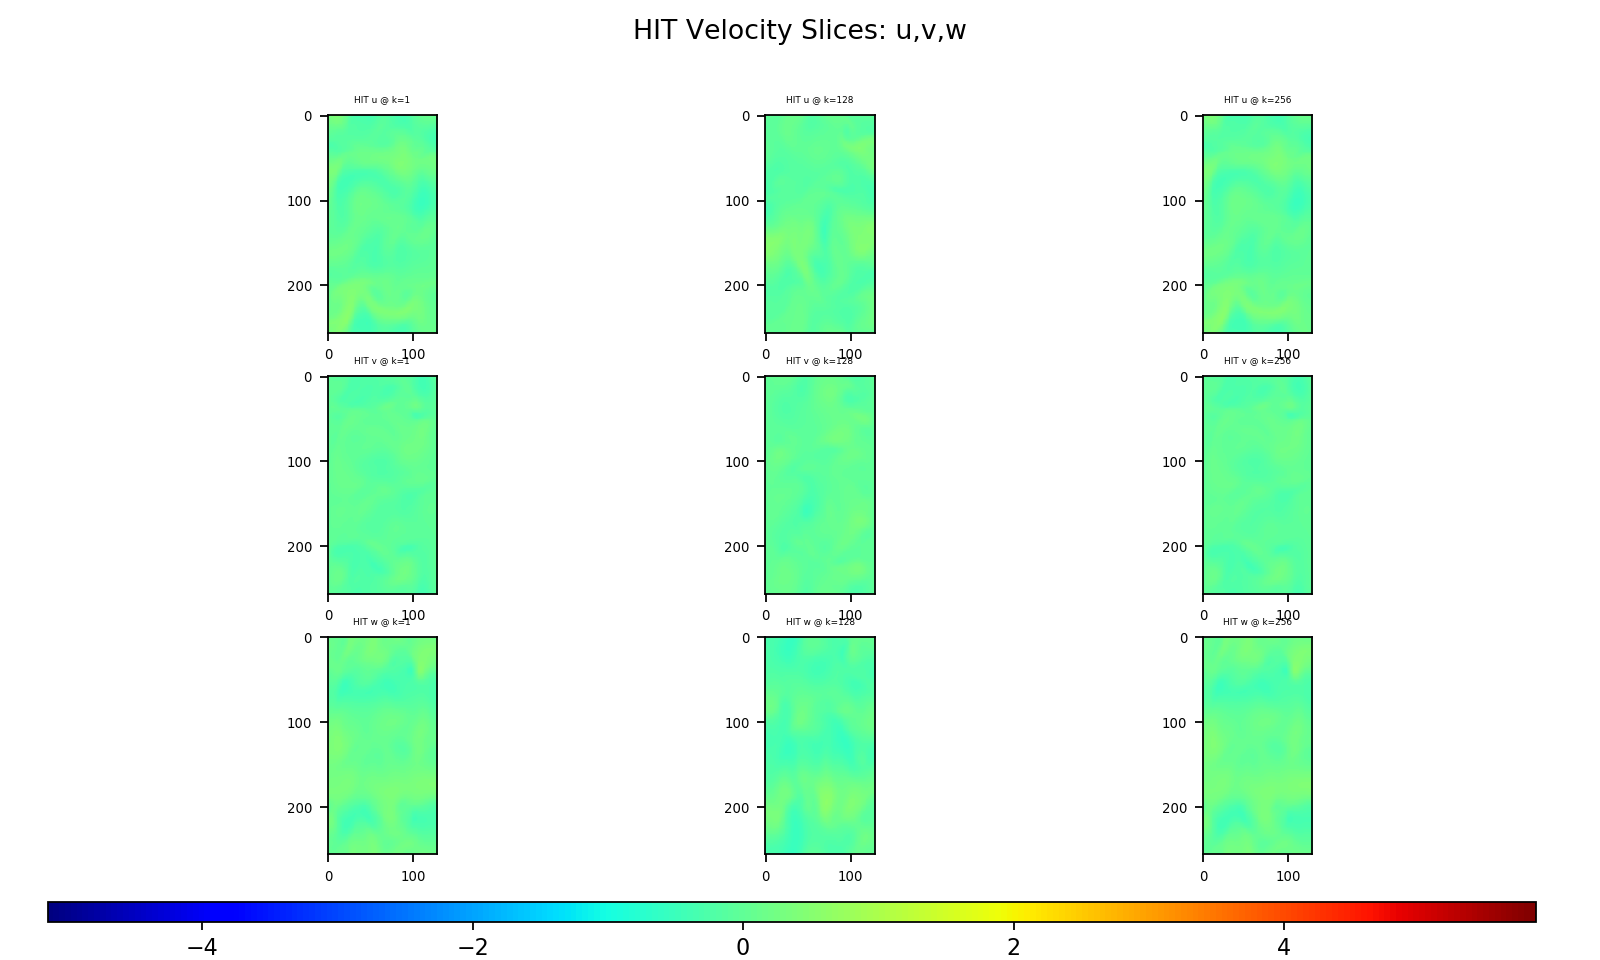
\includegraphics[ width=\linewidth]{./figures/13-hit.png}
	\caption{HIT Velocity Component Slices}
	\label{fig:13-hit}
\end{figure}	

\begin{figure}[H]
	\centering
	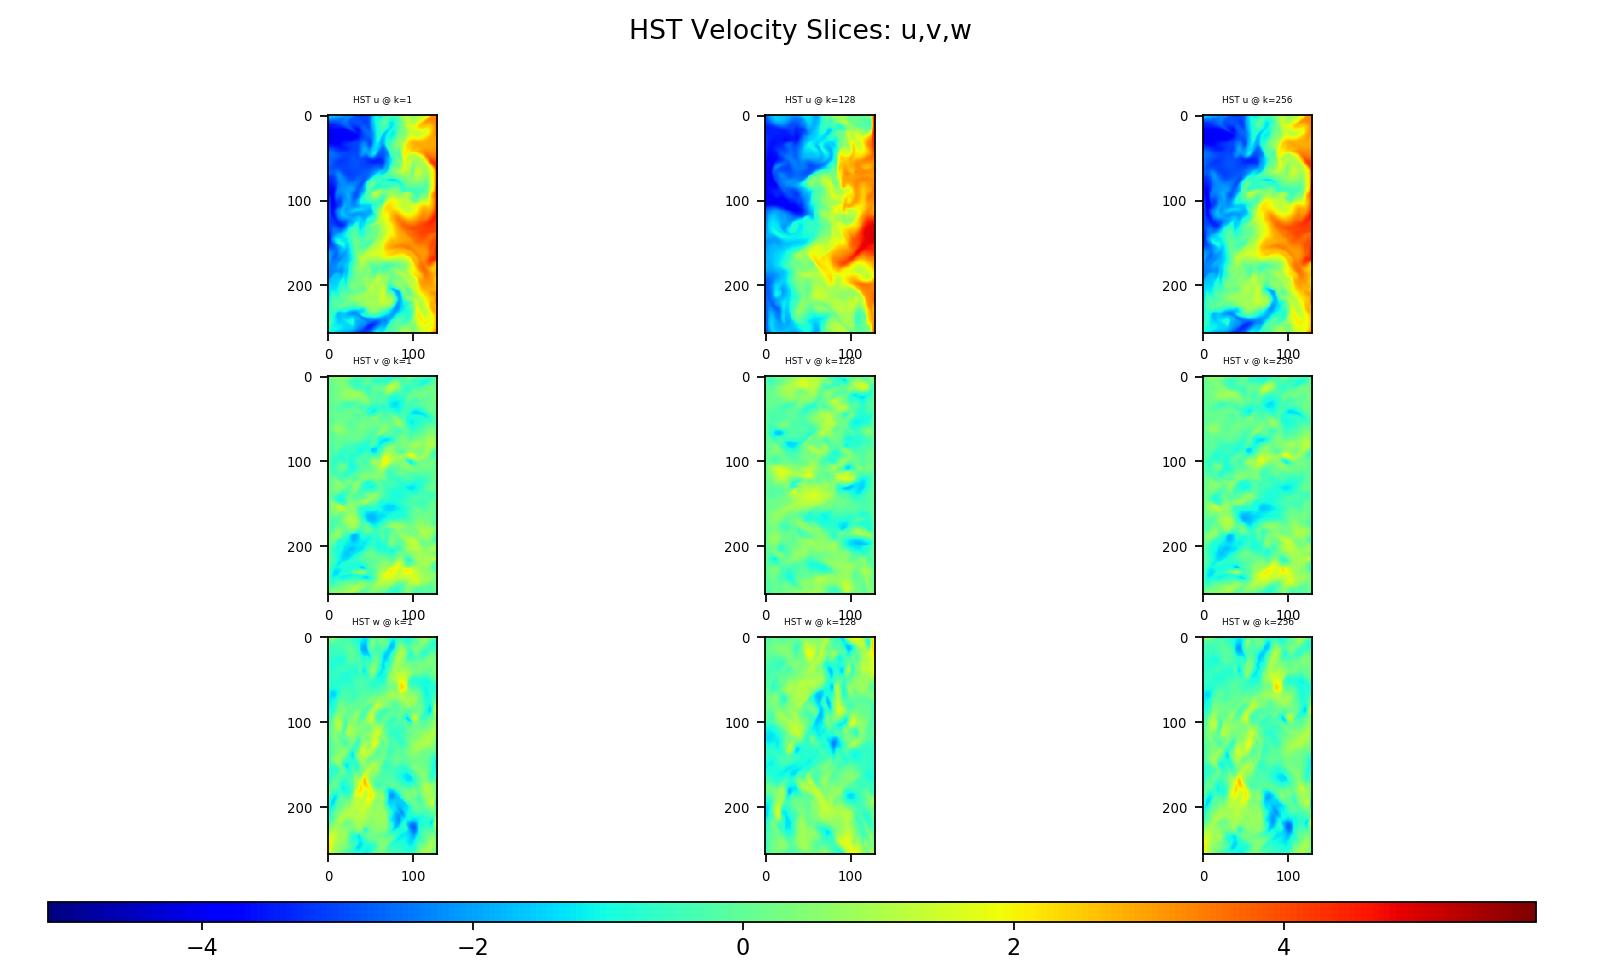
\includegraphics[ width=\linewidth]{./figures/13-hst.png}
	\caption{HST Velocity Component Slices}
	\label{fig:13-hst}
\end{figure}	

\subsection{Spatial Directions}
For the HIT case, one can see from Figure \ref{fig:13-hit} that the fields are spatially homogeneous and the statistics for these fields are expected to be invariant in all directions. 

For the HST case, one sees from Figure \ref{fig:13-hst} that some fields are homogeneous and some are not. The field has strong variation in the y-direction, across the thin axis of the slice. This is due to the shear, where one would expect to see the two opposing layers of velocity. The other directions x and z are homogeneous and their statistics are expected to be invariant. 
\subsection{x-z Averages}
For both the HIT and HST data, x-y averages can be calculated using:
\[
\langle u\rangle_{xz} (j)=\frac{1}{N_xN_z}\sum_{k=1}^{N_z}\sum_{i=1}^{N_x}u(i,j,k)
\]
These values can then be plotted, and seen in Figure \ref{fig:15}. It is interesting to see that the fluctuations in the HIT case are more or less ``random", whereas there is an incredibly strong linear behavior in the HST x-z average of u. This is displaying the shear that is occurring in the domain. Another interesting feature is that the u and w components in the HIT x-z averages appear to be mirrored across some positive-valued line in velocity. Lastly, the v-components of both HIT and HST are quite small, and the w-component in HST is also quite small. The w-component of HST almost has a sinusoidal shape, with the change in concavity being at the location where the x-y u-average changes sign. This could indicate that u-velocity shear is driving flow in the w-direction.

\begin{figure}
	\centering
	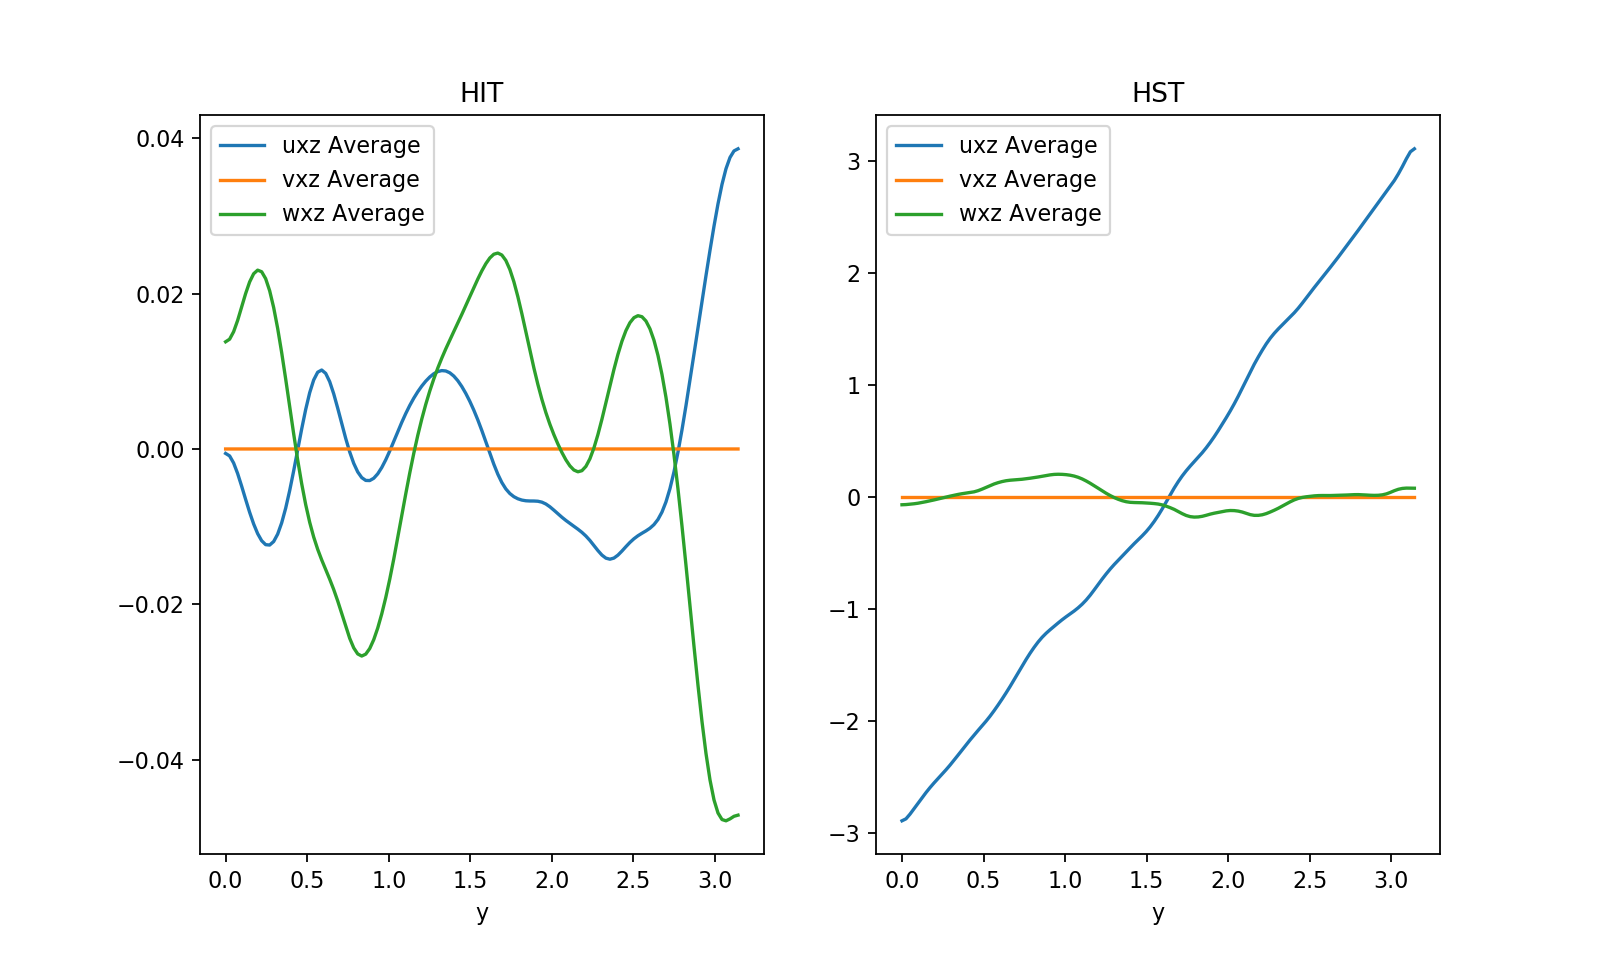
\includegraphics[ width=\linewidth]{./figures/15.png}
	\caption{HIT and HST $u_{i,xz}$ Averages}
	\label{fig:15}
\end{figure}

\subsection{HST Fluctuating Velocity}
The fluctuating velocity can be computed for the HST case utilizing:
\[
u'_i(x,y,z)=u(x,y,z)-\langle u_i\rangle_{xz}(y)
\]
Slices can be taken at k=[1, 128, 256] to create two-dimensional visualizations, seen in Figure \ref{fig:16}. Something really interesting happens when the fluctuating HST velocities are compared with the standard slice velocities in Figure \ref{fig:13-hst}. The v and w components have similar structures in both normal slices and the fluctuation slices, but the u components are significantly different in structure. 

\begin{figure}
	\centering
	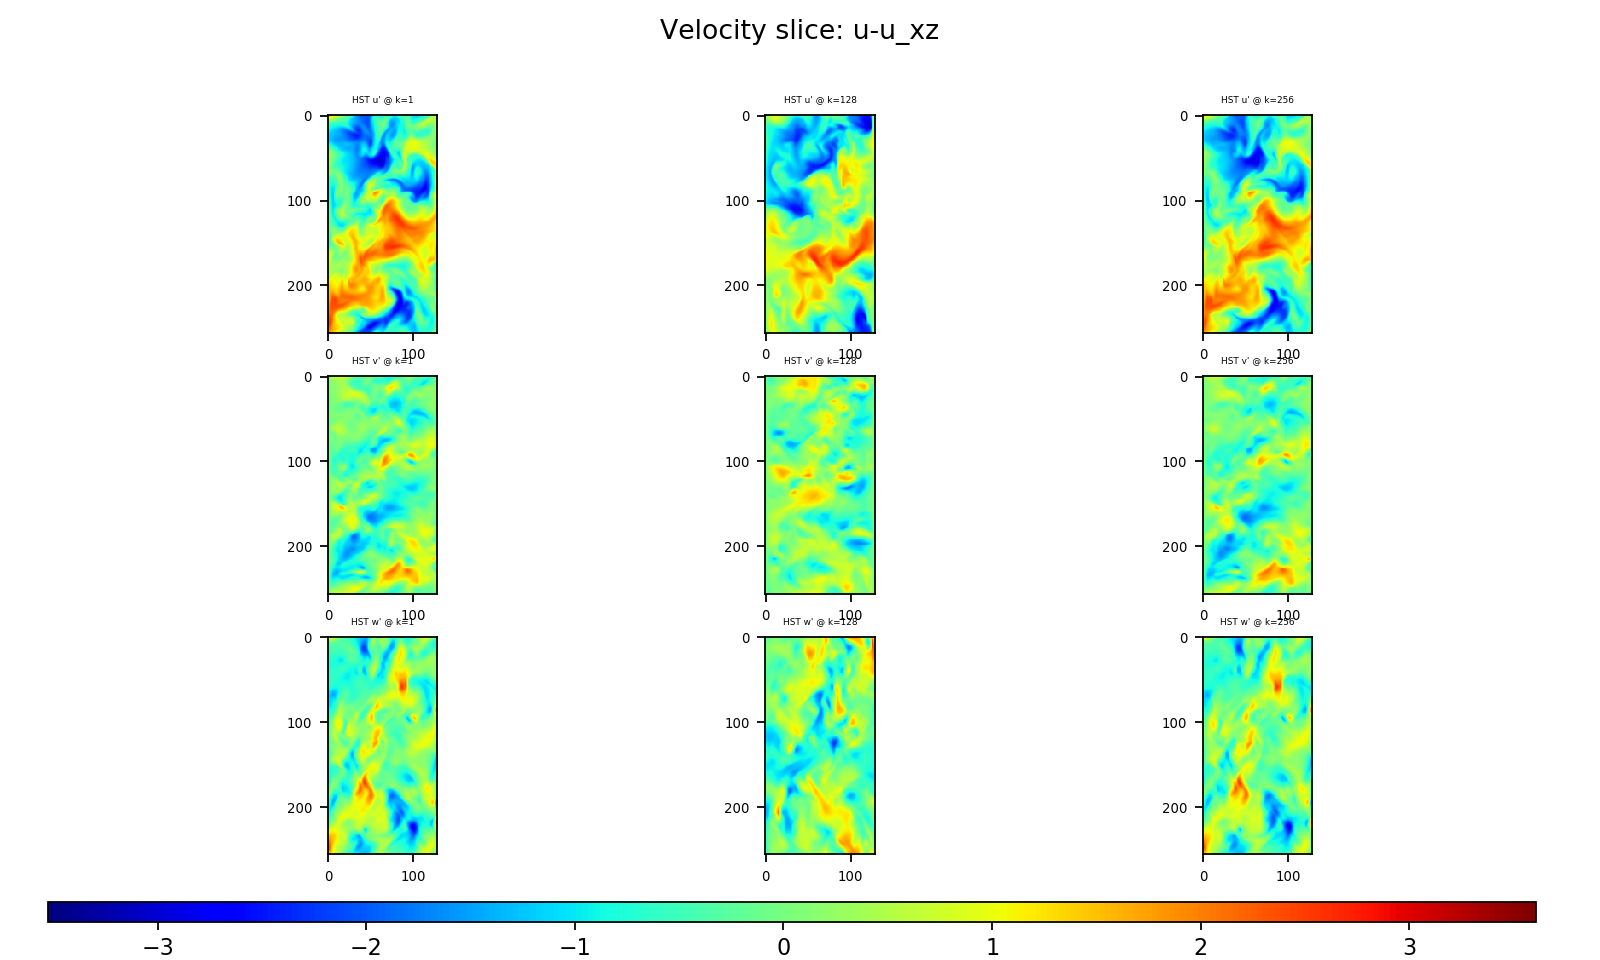
\includegraphics[ width=\linewidth]{./figures/16.png}
	\caption{HST Fluctuating Velocity Slices}
	\label{fig:16}
\end{figure}

\subsection{HIT Fluctuating Velocity}
The fluctuating velocity can be computed for the HIT case utilizing:
\[
u'_i(x,y,z)=u(x,y,z)-\langle u_i\rangle_{xyz}
\]
Note that there is a new average definition here that encompasses the entire volume:
\[
\langle u\rangle_{xyz}=\frac{1}{N_xN_yN_z}\sum_{k=1}^{N_z}\sum_{j=1}^{N_y}\sum_{i=1}^{N_x}u(i,j,k)
\]
When this is done, it obtains the figure seen in Figure \ref{fig:17}. When compared to Figure \ref{fig:13-hit} one can see that the structure and magnitude of the fields themselves don't change all that much. This is likely because the average itself is fairly small due to the nature of the HIT field and therefore the average won't change the fluctuating field significantly. 

\begin{figure}
	\centering
	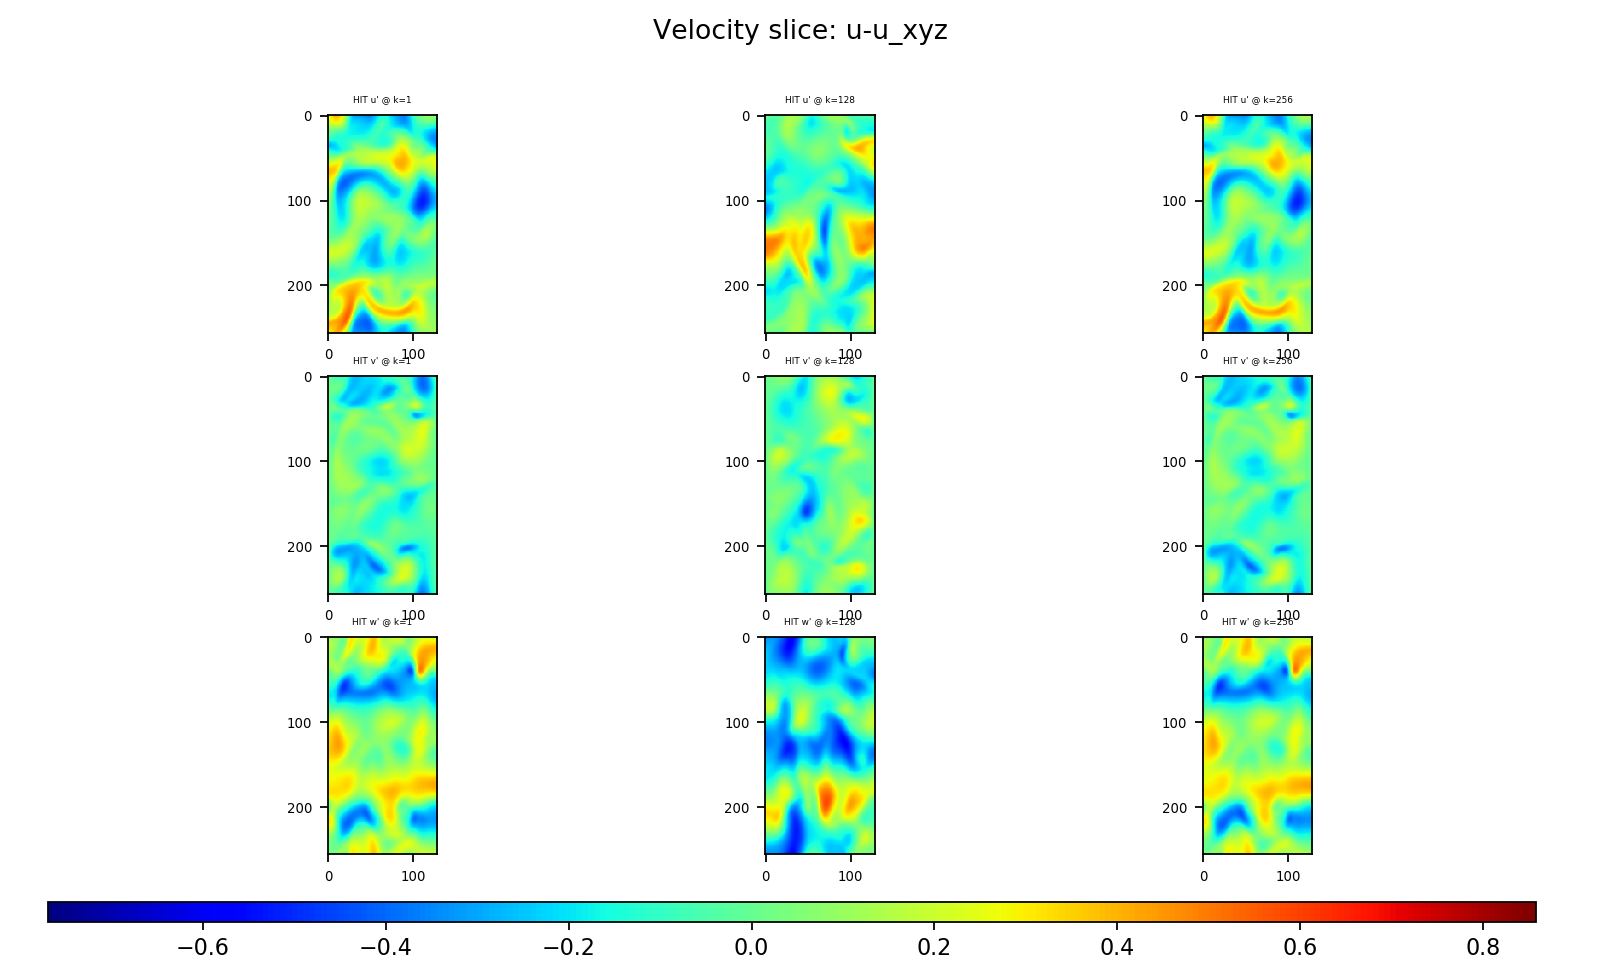
\includegraphics[ width=\linewidth]{./figures/17.png}
	\caption{HIT Fluctuating Velocity Slices}
	\label{fig:17}
\end{figure}

\subsection{Reynolds Stresses}
Now one can calculate the HST Reynolds stresses which are defined as $\langle u_i'u_j'\rangle_{xz}(y)$ since the fluctuating velocities were previously calculated. Additionally, a comparison can be done with the HIT full-volume Reynolds stresses, where instead the full volume average is utilized such that the Reynolds stresses take the form $\langle u_i'u_j'\rangle_{xyz}$. When plotted against each other, the result takes the form in Figure \ref{fig:18}.

\begin{figure}
	\centering
	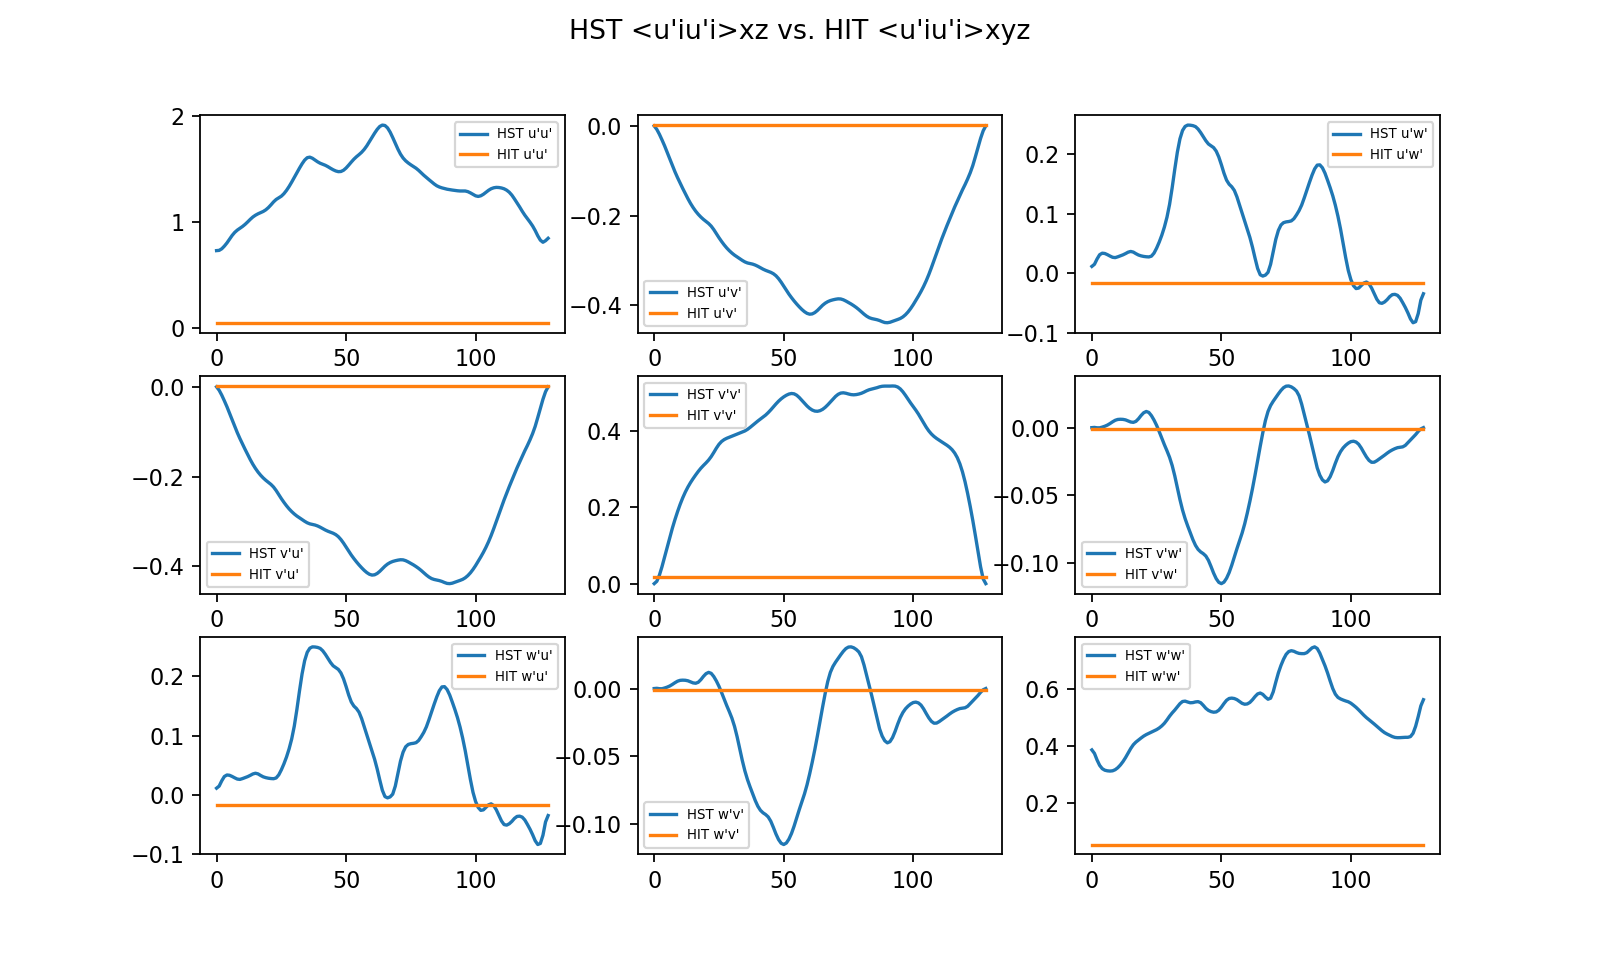
\includegraphics[ width=\linewidth]{./figures/18.png}
	\caption{HIT and HST Reynolds Stresses}
	\label{fig:18}
\end{figure}

Since the average definitions are different, it can be seen that the HST data has fluctuating Reynolds stresses and the HIT data has constant Reynolds stresses. For some components, the HIT Reynolds stress is significantly lower than the HST, such as in in $u'u'$ and $w'w'$. Others, such as $v'u'$ (and it's identical twin as the matrix is symmetric) have the HIT Reynolds stress as the peak value. It is noted that the diagonal components tend to have lower Reynolds stresses whereas the off-diagonal components besides $w'u'$ and $u'w'$ have higher Reynolds stresses for HIT when compared to HST. This makes sense, as stresses should be higher in directions of opposing velocity. Recall that it was mentioned that in the HST case, statistics should be homogeneous except in the y-direction. One can see that in the $w'u'$ and $u'w'$ cases as well as the diagonal the effects of the shear layer are present. 

\subsection{Moments, Skewness, and Kurtosis of $u'$}
The 2nd moment of $u'$ was calculated using the appropriately-defined mean of the nth-moment's nth power of $u'$ for each data set, either HIT or HST. Then $\sigma$ was calculated for each set and skewness was obtained by dividing the third moment by the cube of $\sigma$ and kurtosis was calculated by dividing the fourth moment by $\sigma^4$. The skewness and kurtosis was then plotted for HST and HIT and is seen in Figure \ref{fig:19}, where S represents skewness and K represents kurtosis. In terms of a Gaussian plot, changing the skewness will alter the ``tails" of the PDF plot by changing the lengths of these tails and how far the PDF plot is skewed to one side or another. The larger the skewness, the more the PDF will be ``leaning" to one side, with positive and negative skewness denoting direction. The kurtosis gives effective thickness of these tails, with high kurtosis giving a much spikier, thin PDF whereas a low kurtosis gives a smoother PDF with a rounder shape. The HIT data has relatively low skewness and higher kurtosis, so this means that the resulting PDF won't be leaning much but will be thin. The HST data ranges across many values. Values on the edges should be skewed with higher kurtosis whereas values towards the middle of the data should be more Gaussian. This will be explored next. 

\begin{figure}
	\centering
	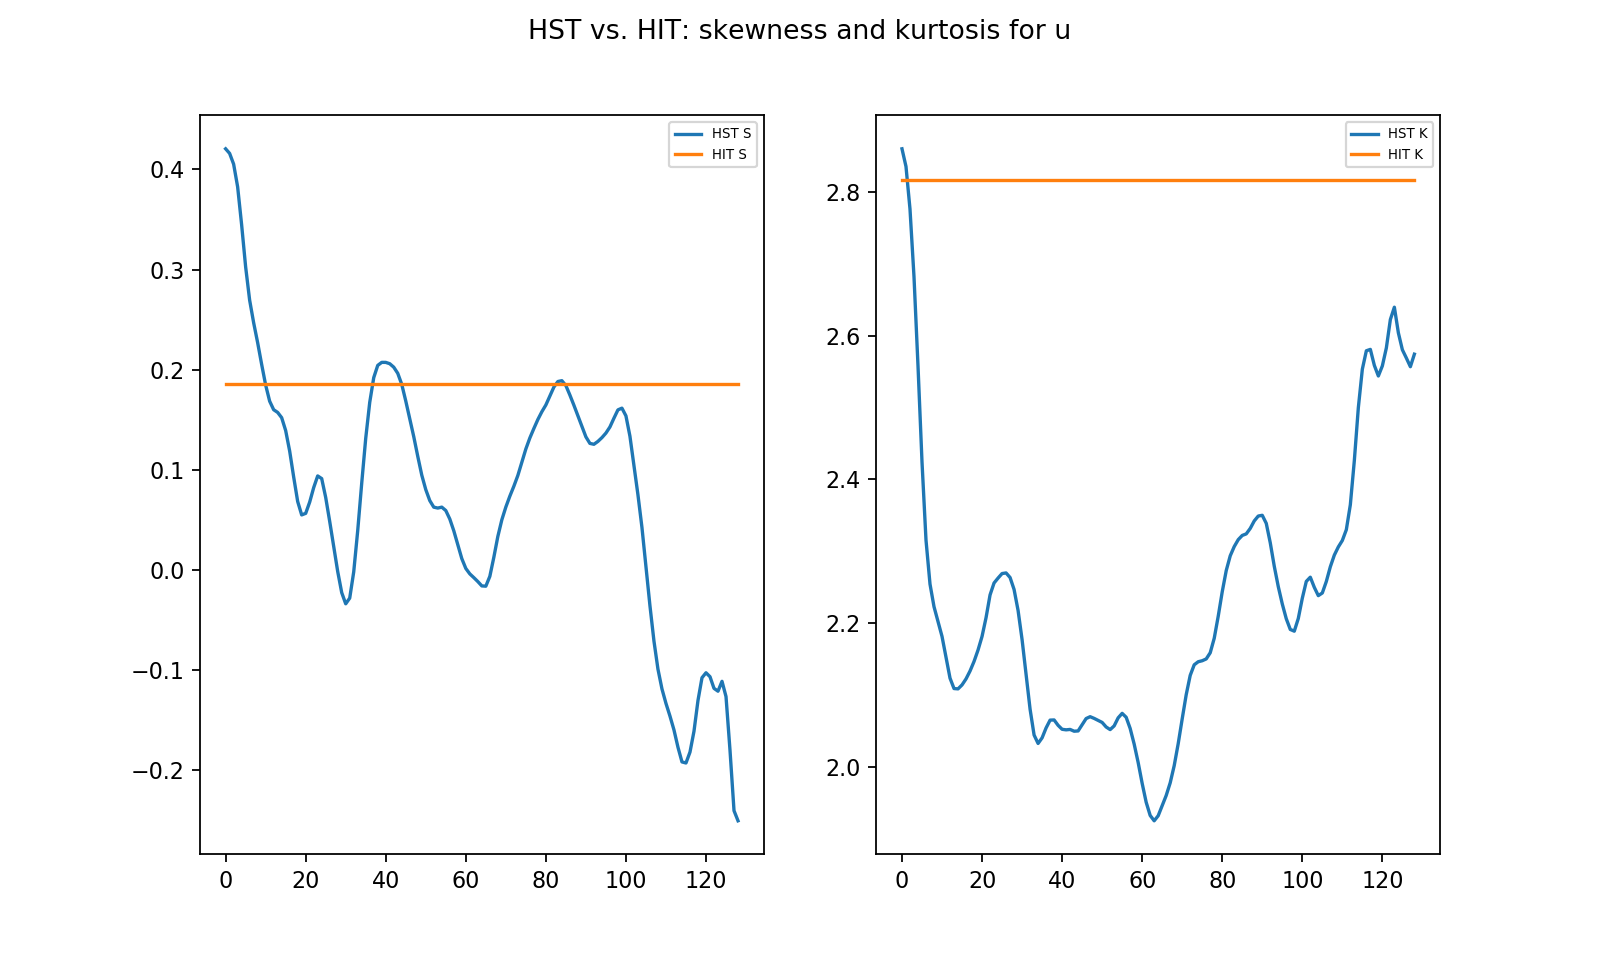
\includegraphics[ width=\linewidth]{./figures/19.png}
	\caption{Skewness and Kurtosis for HST and HIT}
	\label{fig:19}
\end{figure}


\subsection{HST and HIT PDFs}
The probability density functions (PDFs) for the HIT and HST data are plotted in Figures \ref{fig:110-hit} and \ref{fig:110-hst}. For the HST case, the u-velocity components have slightly less kurtosis that the rest of the velocity components. One can also note that the HST v-velocity components have some noticeable skew. The HIT data shows that the u and w components have very Gaussian distributions whereas the v component has considerably more kurtosis. This shows that the v-component field in HIT has some bias towards a very consistent velocity, or likely stillness in the HIT case. The HST PDFs show that there is more variation in velocity across the u-component due to the shear layer(s).


\begin{figure}
	\centering
	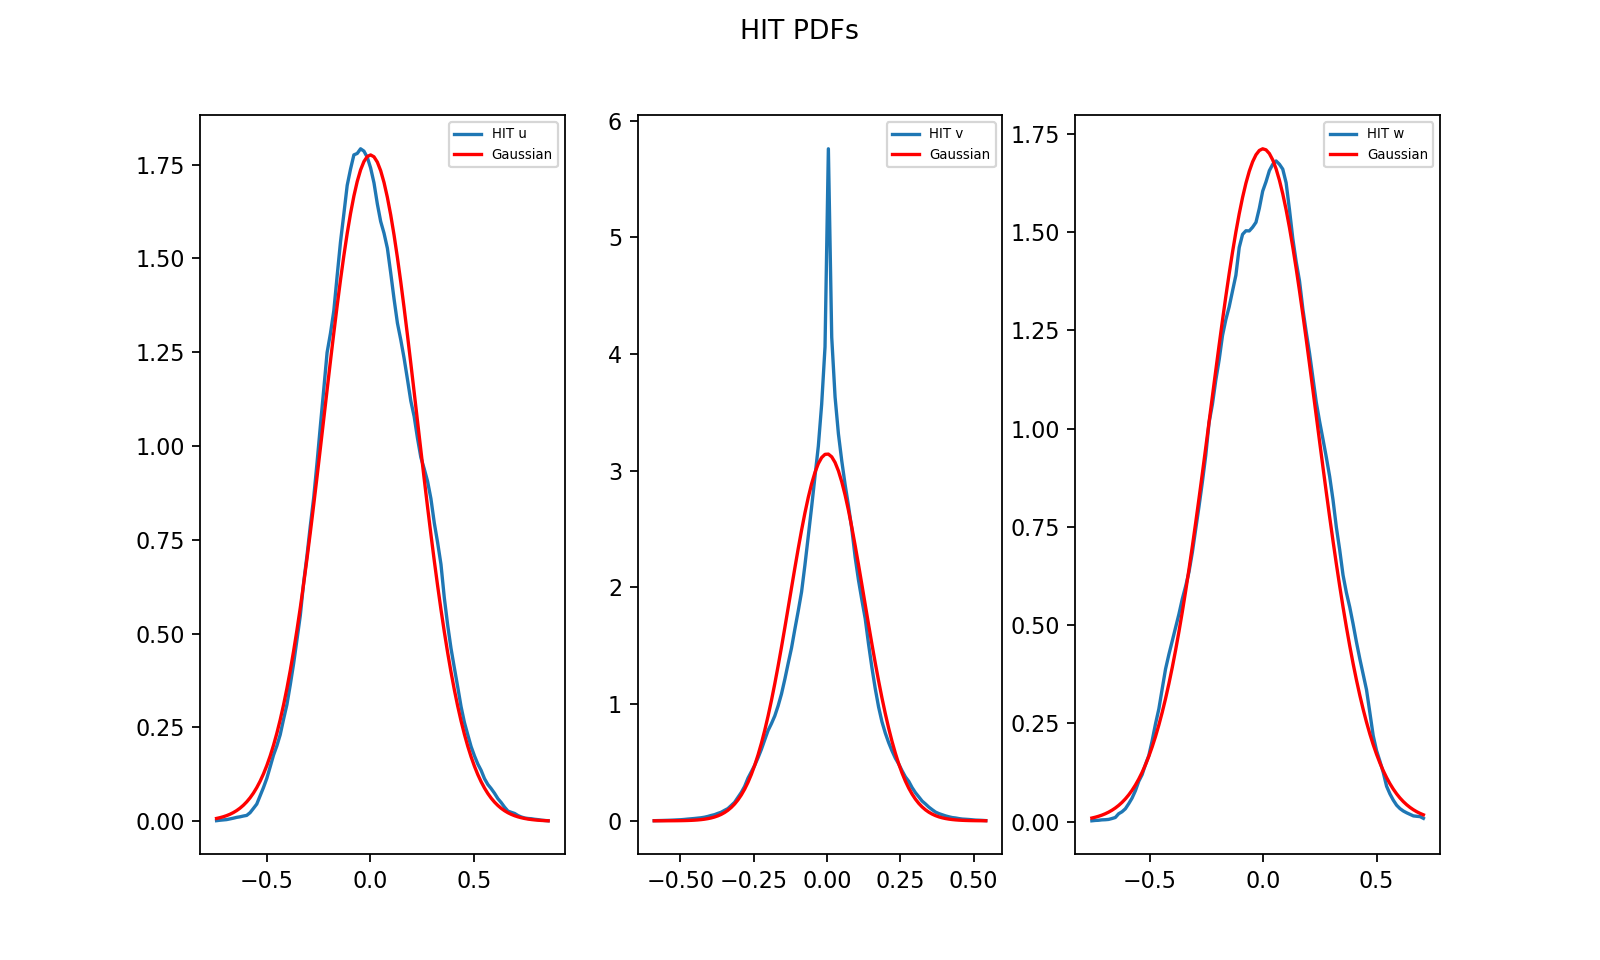
\includegraphics[ width=\linewidth]{./figures/110-hit.png}
	\caption{HIT Data Slice PDFs}
	\label{fig:110-hit}
\end{figure}

\begin{figure}
	\centering
	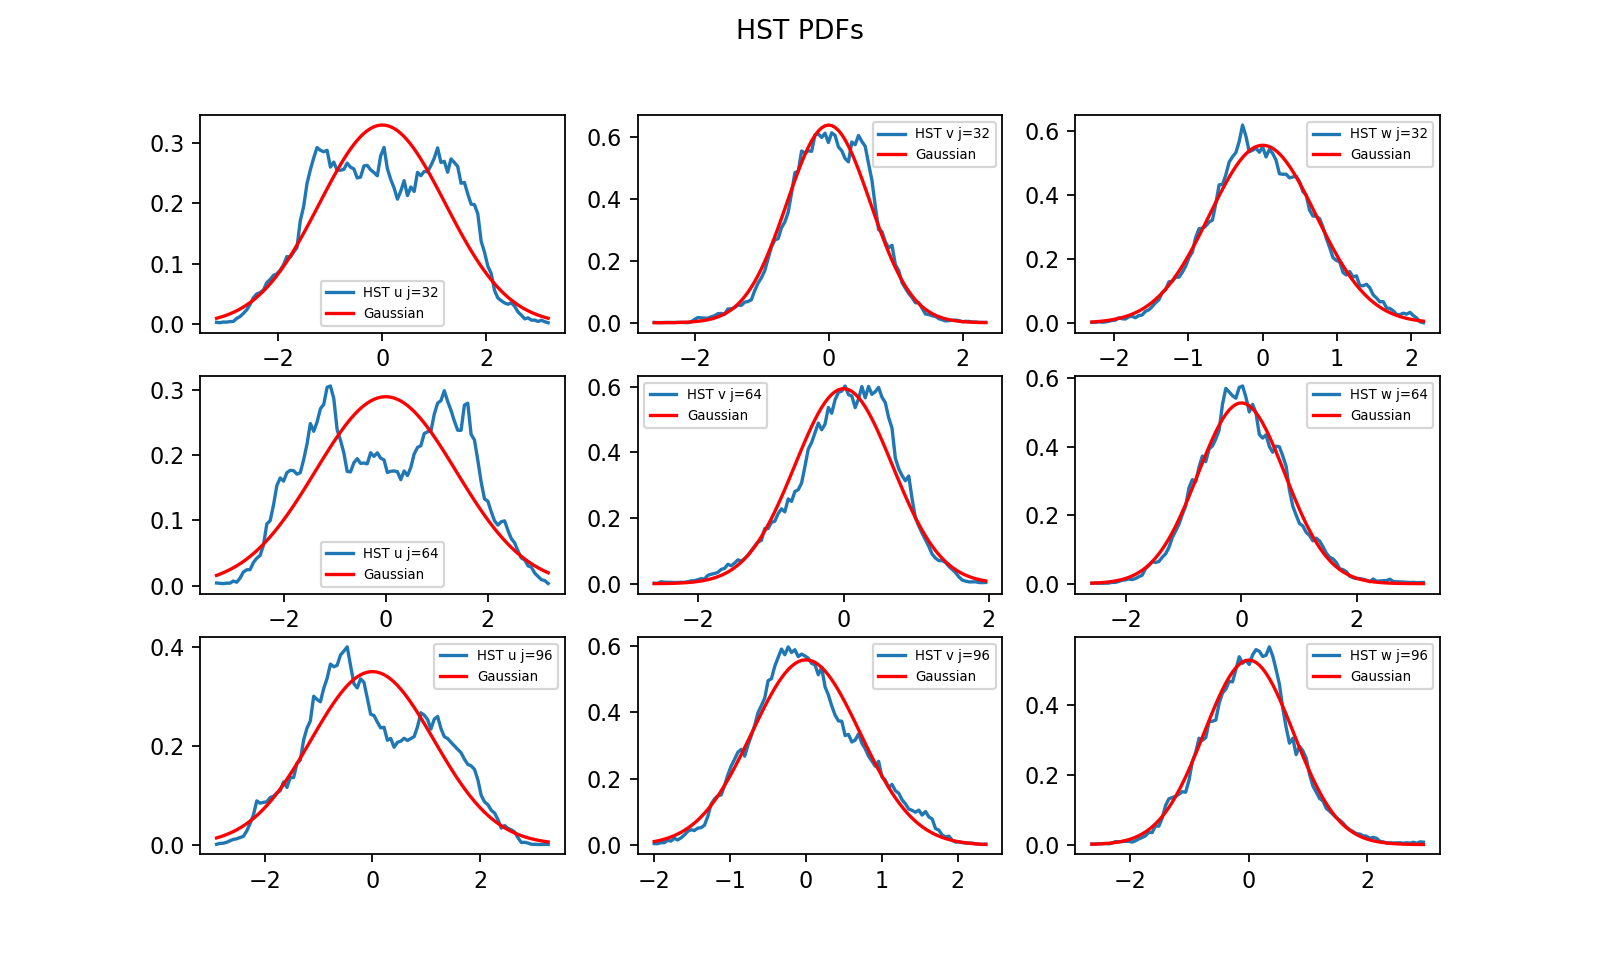
\includegraphics[ width=\linewidth]{./figures/110-hst.png}
	\caption{HST Data Slice PDFs}
	\label{fig:110-hst}
\end{figure}

\section{Problem 2}
This next section will only consider the HIT data. 
\subsection{Velocity Gradient Tensor}
The velocity gradient tensor, 
\[
A_{ij}(x,y,z)=\frac{\partial u_i(x,y,z)}{\partial x_j},
\]
can be calculated for the HIT data for each point in the volume. When volume-averaged, the result is:

\[\langle A_{ij}\rangle_{xyz}=\begin{bmatrix}
 2.74741721e(-08) &  1.24782263e(-02) &  7.31944450e(-06) \\
 5.15238234e(-06) & -3.22052239e(-11) &  1.00500736e(-06) \\
-1.06929170e(-05) & -1.93251442e(-02) & -1.42071821e(-08) \\
\end{bmatrix}\]

Considering HIT, this result seems to make sense as all gradients should be small due to the isotropy. 

\subsection{Fluctuating Velocity Gradient Tensor Field}
The fluctuating velocity gradient tensor field, 
\[
A'_{ij}(x,y,z) = A_{ij}(x,y,z) - \langle A_{ij}\rangle_{xyz}, 
\]
can be computed and the PDFs of the components $A'_{11}$ and $A'_{12}$ are plotted and seen in Figure \ref{fig:22}.

\begin{figure}
	\centering
	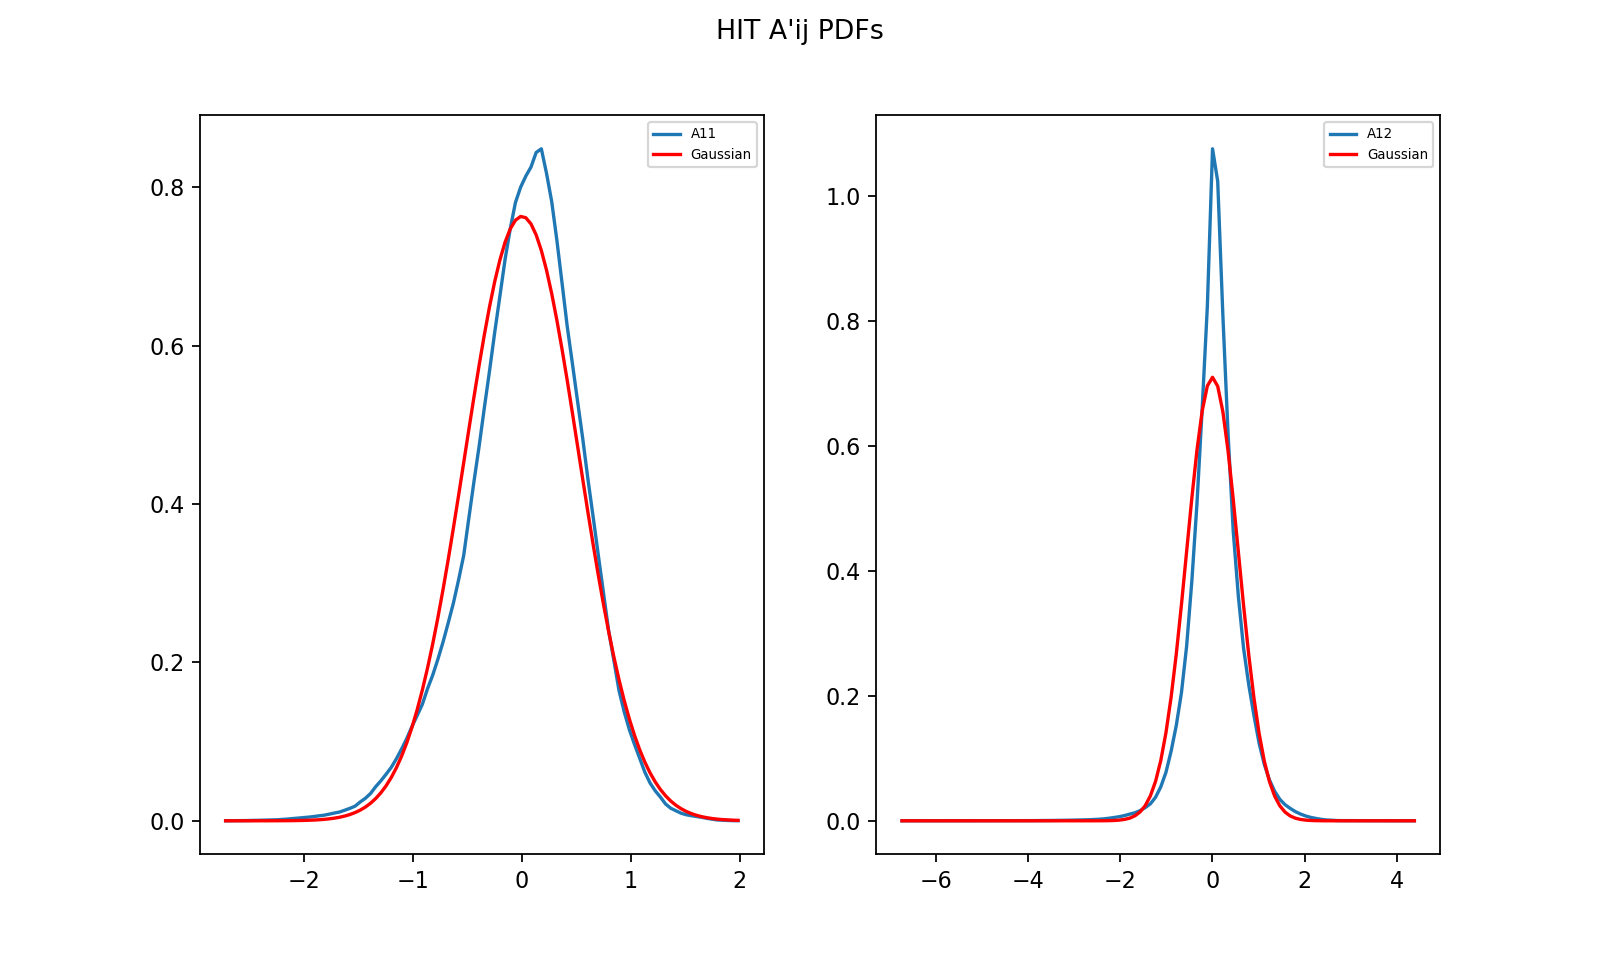
\includegraphics[ width=\linewidth]{./figures/22.png}
	\caption{HIT $A_{ij}'$ PDFs for $A_{11}'$ and $A_{12}'$}
	\label{fig:22}
\end{figure}

The two PDFs are fairly different in shape. $A'_{12}$ has significantly more kurtosis than $A'_{11}$. $A'_{11}$ has similar shape to Gaussian, with close agreement towards the tails and rising edges. $A'_{12}$ also agrees with Gaussian near the tails and rising edges but drastically overshoots the peak. One can see a similarity to the full volume HIT PDFs in Figure \ref{fig:110-hit} for the v-component in velocity and $A'_{12}$ with the strong central peak. The slight stair-step near the peak seen in the w-component velocity HIT PDF lingers in the $A'_{11}$ PDF. 

\subsection{$A'_{11}$ Skewness and Kurtosis}





















































%\bibliography{refs}
%\bibliographystyle{ieeetr}

\end{document}


